\documentclass[../diploma.tex]{subfiles}
 
\begin{document}

	\label{sec:data}

	Для задач, решаемых методами машинного обучения с учителем, к числу которых принадлежат и нейронные сети, важно наличие данных, 
	на которых можно обучать, а затем и тестировать алгоритм.

	\subsection{Сбор данных}

	Так как большая часть имеющихся работ проводила тестирование на данных одного из сайтов системы StackExchange~--- Server Fault \cite{online:serverfault}, 
	который специализируется на теме администрирования веб-серверов,
	то для удобства сравнения результатов мы также решили использовать эти данные.
	Кроме того, этот набор данных удобен тем, что содержит достаточное количество данных для тренировки, при этом с ним удобно работать во время предобработки данных,
	в отличие от базы данных вопросов сайта StackOverflow, размер которой превосходит $50$ гигабайт.

	Для сбора данных использовалась база вопросов Server Fault, 
	размещенная в открытом доступе \cite{online:dataset} и содержащая данные с апреля $2009$ года по март $2018$ года.
	База представляет из себя \texttt{XML}-файл размером $\approx 0.9$ гигабайт, каждая строка которого соответствует либо вопросу, либо ответу.
	В таблице \ref{tab:dataset} кратко описаны атрибуты имеющегося набора данных.

	\vskip 1em
	\begin{table}[ht]
		\centering
    	\begin{tabular}{| l | l |}
    		\hline
    		\textbf{Атрибут}      & \textbf{Описание} \\ \hline
    		Id                    & Идентификатор поста \\ \hline 
    		PostTypeId            & Тип поста \\ \hline
    		AcceptedAnswerId      & Идентификатор выбранного автором ответа (если есть) \\ \hline
    		ParentId              & Идентификатор вопроса, на который был дан текущий ответ \\ \hline
    		CreationDate          & Дата создания поста \\ \hline
    		Score                 & Рейтинг поста \\ \hline 
    		ViewCount             & Количество просмотров поста \\ \hline
    		Body                  & Текст поста в виде \texttt{HTML}-текста \\ \hline
    		OwnerUserId           & Идентификатор автора поста \\ \hline
    		Title                 & Название поста \\ \hline
    		Tags                  & Теги вопроса \\ \hline
    		AnswerCount           & Количество ответов на вопрос \\ \hline
    		CommentCount          & Количество комментариев к посту \\
    		\hline
    	\end{tabular}
		\caption{Описание полей \texttt{XML}-файла с данными}
		\label{tab:dataset}
	\end{table}

	\subsection{Анализ данных}
	\label{subsec:data_analyze}
	
	После анализа было получено, что в имеющемся наборе данных содержится: 

	\begin{itemize}

		\item
		$684$ тысячи постов, из них $257$ тысяч вопросов и $427$ тысяч ответов.

		\item
		$130$ тысяч вопросов ($51 \%$) без выбранного автором вопроса ответа.

		\item
		$28$ тысяч вопросов ($11 \%$), у которых нет ни одного ответа.
	\end{itemize}

	Кроме того, не учитывались вопросы, у которых нет ни одного ответа (так как они не давали никаких новых данных в рамках поставленной задачи), 
	а также вопросы с отрицательным рейтингом, так как вероятнее всего это шумовые данные, 
	в которых заданный вопрос либо плохо сформулирован, либо не соответствует тематике сайта.

	После подобной фильтрации осталось $80$ тысяч вопросов и $180$ тысяч ответов.

	Также было проанализировано содержание текстов вопросов и ответов, в ходе которого выяснилось, 
	что тексты содержат большое количество терминов и слов с опечатками.

	На рисунке \ref{fig:text_lengths} можно увидеть распределения длин текстов вопросов и ответов, 
	которые понадобятся нам в дальнейшем для построения моделей классификаторов.

	Медианным значением длины текста является $500$ символов для вопросов и $350$ символов для ответов.

    \vskip 1em
    \begin{figure}[ht]
        \begin{subfigure}{0.49\linewidth}
        	\centering
        	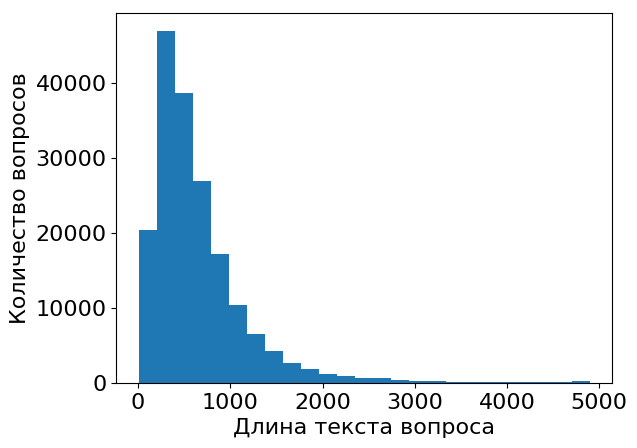
\includegraphics[width=\linewidth]{images/question_lengths.png}
        	\caption{\label{first}Длины вопросов}
        	\label{fig:question_lengths}
        \end{subfigure}
        \begin{subfigure}{0.49\linewidth}
        	\centering
        	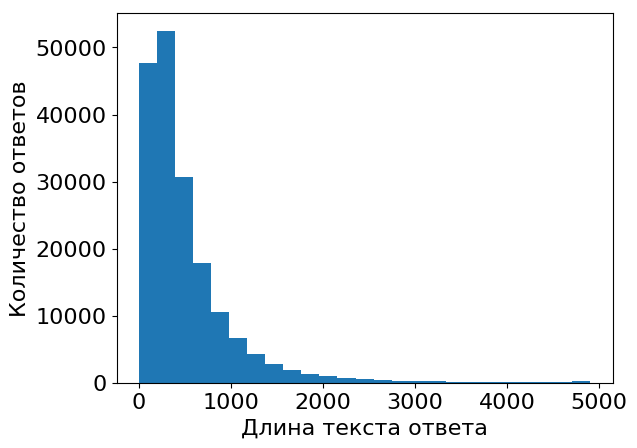
\includegraphics[width=\linewidth]{images/answer_lengths.png}
        	\caption{\label{second}Длины ответов}
        	\label{fig:answer_lengths}
        \end{subfigure}
    	\caption{Распределения длин текстов}
    	\label{fig:text_lengths}
    \end{figure}

	\subsection{Предобработка данных}

	Описанный выше набор данных нужно привести к форме, с которой будет удобно работать в дальнейшем, 
	для этого был написан скрипт на языке Python, который сохраняет данные в формате \texttt{CSV}-файла, каждая запись в котором содержит:
	
	\begin{itemize}

		\item
		Признаки, относящиеся к ответу: идентификатор и текст ответа, был ли ответ выбран автором вопроса, как правильный.

		\item
		Признаки, относящиеся к вопросу: идентификатор, название и текст вопроса, на который был дан текущий ответ.

	    \item
	    Признаки, являющиеся метаинформацией: количество ответов на вопрос, возраст ответа, то есть разница в миллисекундах между датами создания ответа и вопроса.

	\end{itemize}

	Так как в исходном \texttt{XML}-файле текст хранился в виде \texttt{HTML}-кода, был написан обработчик дерева DOM \cite{online:dom}, который:
	\begin{itemize}
	
		\item
		Очищает текст от тегов.

		\item
		Игнорирует содержимое тегов \texttt{del}, \texttt{s} и \texttt{strike}.

		\item
		Заменяет содержимое тега \texttt{code} на специальное слово \texttt{CODE\_LEXEM}.
	
	\end{itemize}

	Все полученные подобным образом тексты были очищены от любых небуквенных символов, приведены к нижнему регистру, разбиты на отдельные слова 
	и сохранены в отдельном \texttt{CSV}-файле.

	\subsection{Разделение данных для эксперимента}

	Для решения задачи машинного обучения итоговая выборка ответов была подразделена на $3$: обучающую, проверочную и тестовую.

	Сначала из всех ответов была выделена тестовая подвыборка размером $20 \%$ от всей выборки, 
	а затем с таким же соотношением оставшаяся выборка была разделена на тренировочную и проверочную.
	Размер подвыборки $20 \%$ был выбран, как один из наиболее распространенных для задач машинного обучения.

	Итого, имеющийся набор данных был разбит на три выборки:

	\begin{itemize}

		\item
		Обучающая выборка: $51000$ ответов.

		\item
		Проверочная выборка: $13000$ ответов.

		\item 
		Тестовая выборка: $16000$ ответов.

	\end{itemize}
	

\end{document}

